\documentclass{llncs}
\usepackage{graphicx}
\graphicspath{ {res/} }
\usepackage{placeins}
\begin{document}
\setcounter{secnumdepth}{3}
\setcounter{tocdepth}{3}
\begin{center}
	
	% Upper part of the page. The '~' is needed because \\
	% only works if a paragraph has started.
	
	\textsc{\LARGE King's College London\\ \small School of Natural and Mathematical Sciences\\ \small Department of Informatics
	}\\[1.5cm]
	
	\textsc{\Large MSc Project Report}\\[0.5cm]
	
	% Title
	\hrule~\\[0.4cm]
	{ \huge \bfseries Smartphone Malware Analysis \\[0.4cm] }
	\hrule~\\[1.5cm]
	
	% Author and supervisor
	\noindent
	\begin{minipage}[t]{0.4\textwidth}
		\begin{flushleft} \large
			\emph{Author:}\\
			Amar Menezes\\(1435460)
		\end{flushleft}
	\end{minipage}%
	\begin{minipage}[t]{0.4\textwidth}
		\begin{flushright} \large
			\emph{Supervisor:} \\
			Dr.~Richard E. Overill
		\end{flushright}
	\end{minipage}
	
	\vfill
	
	% Bottom of the page
	{\large \today}
\end{center}


\begin{abstract}
	 This aim of this report is to survey malware targeting smartphone platforms and to develop an process to detect, analyse and document malware. This process would enable law enforcement, incident response teams and security researchers to efficiently analyse a given malware sample and provide a technical summary of its capabilities, origins, the system weaknesses that it exploits and criminal activities being perpetrated.	 
\end{abstract}
\tableofcontents
\listoffigures

\section{Introduction} \label{Intro}
	Traditionally malware authors have targeted personal computers, workstations and servers. Mainly because they were potentially rich stores of sensitive information. Mobile phones however were mainly used for communication and did not offer much incentive for malware authors. Over the years smartphones and tablets have started replacing personal computers. People now use their smartphones not just to make calls and send messages, but for a host of other applications such as e-commerce transactions, data storage, navigation, socializing etc. Our smartphones now house a lot of our personal and financial information. This provides a huge incentive for malware authors to focus their efforts on attacking smartphones.\\

	In the pre-smartphone era mobile phone vendor used its own proprietary operating system and the phones capabilities itself were limited. Unlike the pre-smartphone era today's smartphones have far greater capabilities from their sophisticated hardware and their constantly improving platforms. Platform capabilities are expposed via APIs which allow applications to be developed by third party vendors. The majority of smartphones today run on one of the three platforms which are Android\cite{android-home}, iOS\cite{iOS-home} and Windows Phone\cite{WindowsPhone-home}. As of Q1 2015, Android holds the largest market share at 78.0\%, followed by iOS with 18.3\% with Windows Phone, BlackBerry and others making up for the remaining 3.7\% share \cite{idc-smartphone-marketshare}.
	
	
\section{Background} \label{related_work}
This section describes work that has been done on malware analysis for desktops and personal computers and the evolution of malware analysis for smartphones. This would include the investigation process, sandboxes and automated tools.\\
We also talk about the challenges with smartphone malware analysis	
\subsection{Malware attack goals}
Suarez-Tangil et al.\cite{suarez2014evolution} categorised malware based on their attack goal and behaviour, method of distribution and privilege acquisition.\\\\
Attack goals and behaviour are summarised as
\begin{enumerate}
	\item[]{\textbf{Fraud:} Such as sending SMS/Calling premium numbers or holding device data or functionality ransom.}
	\item[]{\textbf{Sabotage:} Such as destroying data or rendering the device unusable.}
	\item[]{\textbf{Theft:} Exfiltration of user information (contact lists, messages, IMEI/IMSI numbers, call/location history etc) and/or user credentials (banking, social accounts, email, corporate accounts)}
	\item[]{\textbf{SPAM:} Agressive Adware}
	\item[]{\textbf{Service Misuse:} Such as snooping, spying or tracking of the user by exploiting device sensors. Another example is running a botnet without the users knowledge.}\\
\end{enumerate}

\subsection{Modes of distribution}
Methods of distribution and infection were categorized as follows
\begin{enumerate}
	\item[]{\textbf{Market to Device:} An attacker uses an app market to upload his/her malicious application. If markets are not policed for malicious content users are at risk of getting infected.}
	\item[]{\textbf{App to Device:} In this mode of distribution the attacker uses a vulnerable application to distribute his/her malicious application.}
	\item[]{\textbf{Web to Device:} This mode of distribution exploits vulnerabilities in web browsers to distribute malicious content.}
	\item[]{\textbf{SMS to Device:} Malware uses SMS/MMS to distribute malicious payloads. This was a popular strategy targeting the SymbianOS.}
	\item[]{\textbf{Network to Device:} This strategy exploits platform vulnerabilities or misconfigurations. Distribution uses either Device to Device (D2D) propagation or Cloud to Device (C2D) propagation.}
	\item[]{\textbf{USB to Device:} Malware infects devices when they are connected to an infected computer via a communication port usually USB.}\\
\end{enumerate}
Privilege acquisition is generally achieved via two methods
\begin{enumerate}
	\item[]{\textbf{User Manipulation:} An unsuspecting is tricked into granting privileges to malware. User manipulation is achieved via Social Engineering, use of repackaged applications from third-party sources, etc.}
	\item[]{\textbf{Technical Exploitation:} Here privileges are acquired by exploiting platform vulnerabilities or misconfigurations. Although vulnerabilities differ across platforms, most common attacks include API vulnerabilities, buffer overruns, injection attacks, protocol vulnerabilities etc.}
\end{enumerate}

\subsection{Malware capabilities} \label{capabilities}
Faruki et al. \cite{farukiandroid} categorised malware based on their capabilities within the context of smartphones.
\begin{itemize}
	\item[]{\textbf{Trojan:} Malicious apps that appear to have a benign purpose to the user, while performing harmful activities without the user being aware. Trojans are typically used in the exfiltration of sensitive data such as user credentials, contacts, messages etc. SMS Trojan families send SMS's to premium rate numbers without the user being aware.}
	\item[]{\textbf{Backdoors:} This type of malware infects systems exploiting platform weaknesses. Backdoors typically use root exploits to escalate privileges and evade detection.}
	\item[]{\textbf{Worm:} Malicious apps that create copies of itself which it distributes to other systems via networks and/or removable media.}
	\item[]{\textbf{Botnets:} These apps compromise the device to create a Bot, which forms part of a network of other such bots called a botnet. Bots are controlled by a Command and Control server and are used for malicious activities ranging from data exfiltration to denial of service attacks.}
	\item[]{\textbf{Spyware:} These apps perform malicious activites such as monitoring calls, contacts, messages, location, etc. It can also send this data to a remote server controlled by the attacker.}
	\item[]{\textbf{Adware:} These apps spam the user with unsolicited advertisements and notifications. These can create shortcuts on the home screen, steal bookmarks, and impair effective usage of the device.}
	\item[]{\textbf{Randsomware:} This type of malware locks the user out of his/her data and demands a ransom to unlock the data.}
\end{itemize}

\subsection{Current research in Malware detection}
This section describes the work done by researchers on mobile malware analysis, tools and sandboxes.

\subsection{Limitations of current technologies}
This section describes the limitations of the existing methodologies and tools.

\section{Smartphone Platforms} \label{platforms}
\subsection{Android}
Android is an open source smartphone operating system being currently developed and maintained by Google Inc. and promoted by the Open Handset Alliance (OHA). Android was originally conceived by Andy Rubin, Chris White, Nick Sears and Rich Miner at Android Inc in October 2003. Android Inc was later acquired by Google Inc in August 2005. The Open Handset Alliance is a consortium of 84 companies led by Google consisting of mobile handset manufactures, software developers, chipset manufactures and a few telecommunication companies \cite{open-hadset-alliance}.

\subsubsection{Ecosystem}
The first Android smartphone was the HTC Dream running Android 1.0 released in September 2008, followed by an upgrade to Android 1.1 in February 2009. From version 1.5 onwards Android releases were codenamed with names of deserts and pastries. The table below summarises the different Android releases and their codenames.
\begin{center} 
\begin{tabular}{|l|c|c|c|r|}       %lcr = allignment of the individual cols
	%| puts a line in between them
	\hline %a line at the top
	Version & Codename & API Level & First Release & Distribution \\
	\hline\hline %puts a line under first row
	1.5 & Cupcake & 1 & April 2009 & \textless 0.1\% \\
	1.6 & Donut & 4 & September 2009 & \textless 0.1\% \\
	2.0.x and 2.1 & Eclair& 5 & October 2009 & \textless 0.1\% \\
	2.2.x & Froyo & 8 & May 2010 & 0.3\% \\
	2.3.x & Gingerbread & 10 & December 2010 & 5.6\%\\
	3.x & Honeycomb & 11 & February 2011 & Unavailable \\
	4.0.x & Ice Cream Sandwich & 15 & October 2011 &  5.1\%\\
	4.1.x, 4.2.x and 4.3.x & Jelly Bean & 16-18 & July 2012 & 37.4\%\\
	4.4.x & KitKat & 19 & October 2013 & 39.2\% \\
	5.x & Lollipop & 21-22 & November 2014 & 12.4\%\\
	\hline %a line at the bottom
\end{tabular}
\end{center}

The ecosystem is not just about the distribution of andriod versions but also comprises of hardware vendors, carriers and developers. Hardware vendors consists of CPU manufacturers, System-On-Chip(SoC) manufacturers and device manufactures.
\begin{itemize}
	\item{\textbf{CPU Manufacturers:} A majority of Android devices run on an ARM architecture based processor due to its low power consumption. ARM Holdings does not manufacture CPUs but licences its technology as intellectual property. The ARMv7 instruction set is common in todays android smartphones.
	In 2011, Google partnered with Intel to support Intel processors on Android. Intel started the Android on Intel Architecture (Android-IA) project to enable Android on Intel processors. Like ARM, MIPS Technologies has licensed its processor architecture designs to other manufacturers. MIPS based proccessors are found in tablets, set-top boxes, media players etc.}
	\item{\textbf{SoC Manufactures:} System-On-Chip are components that include a CPU, GPU, RAM, I/O controllers, baseband processors all included on a single silicon chip. Manufacturing SoCs are more cost effective and power efficient as compared to individual components. The main SoC families are Tegra from nVidia, OMAP from Texas Instruments, Exynos from Samsung and Snapdragon from Qualcomm.}
	\item{\textbf{Device Manufactures:} The final handset the consumers purchase is designed and built by device manufacturing companies. Some well known companies include Samsung, LG, Motorola, HTC and Sony. Device manufactuers tend to customize the Android framework to differentiate themselves from the competition. However these customizations could lead to vulnerabilities in the Android framework. Since the Android framework is licenced under the Apache 2.0 Licence, modified binaries can be redistributed without releasing the source code.}
\end{itemize}

Carriers provide voice and data services to smartphone customers. Some carriers also partner with device manufacturers to provide phone deals to customers. Carrier deals customize the phones firmware before being made available to customers.

Lastly developers form a significant part of the Android ecosystem. Developers contribute to the Android project as well as building applications for the Android platform. Some android enthusiasts also develop custom firmware projects also known as ROMs for different android devices. The most popular of these projects is CyanogenMod \cite{cyanogenmod}.

\subsubsection{Software Stack}
The Android platform architecture consists of five components \ref{fig_android_stack}. Android applications, the Android framework, the Android Runtime, User-space native code and the Linux kernel.
\begin{figure}[h]\label{fig_android_stack}
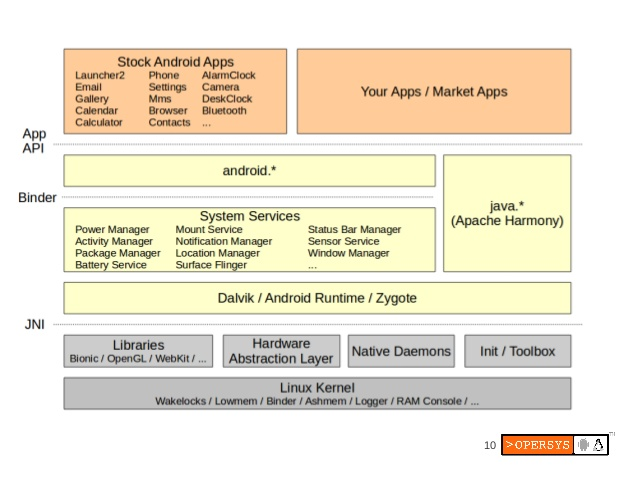
\includegraphics[width=\textwidth]{android_stack}
\centering
\caption{Android platform architecture\cite{android_stack}} 
\end{figure}

At the top of the software stack are the Android applications. Application developers use the Android API to build applications that the end user interacts with. Applications found on a device are either system apps which come installed with the stock OS and user installed apps which can be installed from the Google Play Store or other sources.
The Android Framework provides application developers a rich API to access the devices capabilities. The framework allows developers to manage UI interaction, access to media storage, access to device peripherals such as the baseband controller, camera, GPS, wifi controllers, inter process communication, etc.
The Android Framework and Android applications are developed in Java. Applications are compiled into Dalvik Executables (or dex files) which are then interpreted by the DalvikVM. The DalvikVM is a register based virtual machine that executes applications written for Android. The DalvikVM forms an integral part of the Android Runtime and provides a layer of abstraction to the underlying operating system. Android 4.4 (KitKat) introduced a new runtime called Android Run Time (ART) as an experimental alternative. Unlike Dalvik which used Just-In-Time compilers to convert dex bytecode into native code, ART uses Ahead-Of-Time compilers to compile the application into native code upon their installation. In Android 5.0 ART replaced Dalvik as the sole Android runtime.
In addition to the Android Framework, developers can access system services (eg. dhcpd, wpa\_supplicant,etc) and system libraries(eg bionic libc, WebKit, OpenSSL, etc) via user-space native code components. These components allow access to services and libraries that talk directly to the Linux kernel and avoid the overhead of the Android Runtime. Low-level native code operations are employed when application performance is paramount.
The final component of the Android stack is the Linux kernel. The kernel has been modified to operate smartphone hardware. Kernel drivers control device peripherals, network components, process management and file system access. Some of the android specific kernel drivers are wakelocks for power management, ashmem for anonymous shared memory, alarms, paranoid networking and Binder. Paranoid networking and Binder are important from a security perspective as the former restricts access to network sockets to applications based on their permission set and the latter implements Inter Process Communication (IPC) and an associated security mechanism. 

\FloatBarrier
\subsubsection{Application structure and components}
Android applications are distributed in via APK (Android PacKage) files. An apk is a zip archive of several files and folders. An android application package has a folder structure as shown in \ref{fig_apk_struct}
\begin{figure}[h] \label{fig_apk_struct}
	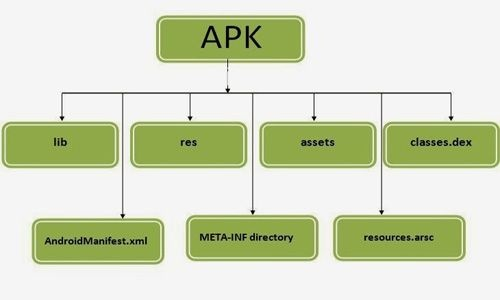
\includegraphics[width=\textwidth]{apk_structure}
	\centering
	\caption{Android package structure\cite{apk_structure}} 
\end{figure}
\begin{itemize}
	\item[]{\textbf{AndroidManifest.xml:} This file includes the application meta-data such as package name, minimum and maximum supported API level, permissions requested, libraries used and application components such as Activities, Services, Broadcast Receivers and Content Providers.}
	\item[]{\textbf{classes.dex:} This file contains the Dalvik bytecode to be executed by the DalvikVM.}
	\item[]{\textbf{META-INF:} This folder contains the application certificate and a list of files included in the apk along with their SHA-1 hashes.}
	\item[]{\textbf{lib:} This folder contains native binaries that the application uses. These binaries are stored in sub-folders, created for each supported CPU architecture.}
	\item[]{\textbf{assets:} This folder contians application assets that can be retrieved by the AssetManager class.}
	\item[]{\textbf{res:} This folder contains resources that are not compiled into the resources.arsc file. These include icons, images, UI layouts, menus, etc.}
	\item[]{\textbf{resources.arsc:} This file contains resources that are pre-compiled, for example application strings.}
\end{itemize}

\FloatBarrier

Having discussed the package structure we now look at the top level components of an android application. App components are entry points for the system to access the application. There are four different components with a distinct lifecycle. These are summarised below \cite{android-fundamentals}.
\begin{itemize}
\item[]{\textbf{Activities:} These components make up the user interface of the application. An application can have more than one Activity and these are all listed in the AndroidManifest.xml file. Activities are also capable of returning results to its caller.}
\item[]{\textbf{Services:} Services are similar to Unix daemons performing background tasks without the need for user interaction. Services usually performing long-running operations or operations for remote processes. For example playing audio in the background or downloading data over the internet.} 
\item[]{\textbf{Broadcast Receivers:} These components listen to events generated by the Android Operating system or application broadcast  events. Examples of system generated broadcast events are BOOT\_COMPLETED, SMS\_RECIEVED, etc.} 
\item[]{\textbf{Content Providers:} These components provide an interface to allow sharing of stored data with other applications. Data stored on the file system, Cloud, databases etc can be queried via Content Providers. An example the Android system provides a Content Provider to access the users contacts.}
\end{itemize} 

Activities, Services and Broadcast Receivers are activated via asynchronous messages called Intents. Intents request a particular action from a component and may specify the URI of data to act on. Content Providers are not activated via Intents, rather they are activated when targeted by a request.

\subsubsection{Security model}
This section just summarises the most significant aspects of the android security model extracted from \cite{Drake:2014:AHH:2614422}, \cite{Elenkov:2014:ASI:2631372} and \cite{Tyrone:2015:MAHH}
\paragraph{\textbf{Permission model}}
Android uses two distinct but co-operating permission models as part of its security model. These two models are enforced by the Linux kernel and the other by the Android Runtime and Framework. The Linux kernel uses users and groups to enforce permissions on the file system and other android resources. This permission model is commonly refereed to as the Android Sandbox.\\
The Android Runtime and Framework defines a set of permissions which limit the abilities of the application. These permissions are listed in the AndroidManifest.xml file and are first displayed to the user when the application is installed.

\paragraph{\textbf{Android Sandbox}}
Like traditional Linux platform Android uses user ID (UID) and Group ID (GID) paradigm, however it does not have a \textit{passwd} or \textit{group} files. It was reasoned that there would be only one user to the system (i.e. the owner of the smartphone) and so the UIDs were assigned to individual applications known as Android IDs (AID), instead of to each user on the system. Certain AIDs are reserved for privileged and system-critical applications such as those belonging to the system/user group. Like in Linux each process has its own memory space and cannot interfere with another running process. In addition to process isolation the Android Sandbox also achieves data isolation by assigning a each application a dedicated data directory with read and write permissions.

\paragraph{\textbf{Android Permissions}}
In order to allow access to hardware, system services, data storage, Internet connectivity etc., Android grants additional access rights by way of \textit{API Permissions}. Permissions requested by an application are listed in the AndroidManifest.xml file. These permissions are granted to the application at the time of installation and once granted cannot be revoked. Some API permissions map to low-level kernel permissions for example the API permission \textit{android.permission.INTERNET} which grants the application access to the Internet maps to the kernel managed group \textit{inet} which grants users the ability to open sockets.

\paragraph{\textbf{Protection Levels}}
Each API permission has an associated \textit{protection level}. Some permissions are more sensitive than others and protection levels define the conditions under which the applications are granted permissions. The table below summarises the four protection levels defined by Android.
\begin{center} 
	\begin{tabular}{|cp{0.5\textwidth}|cp{0.5\textwidth}|}      
		\hline 
		Protection Level & Description \\
		\hline 
		normal & This is the default protection level and generally associated with permissions that have a low risk to the system and other applications  \\
		\hline
		dangerous &  Permissions that could allow access to sensitive data or access the devices hardware, have a protection level set as dangerous. \\
		\hline
		signature & Permissions with this protection level are only granted to applications that have been signed by the same key as the application that declared the permission. \\
		\hline
		signatureOrSystem &  Permissions with this protection level are granted to applications that have either the same signing key or are part of the system image.\\

		\hline %a line at the bottom
	\end{tabular}
\end{center} 

\paragraph{\textbf{Code signing}}
Android mandates that every application be signed before it can be installed on the system. Signing is done with digital certificates whose private key is held by the authors of the application. Code signing establishes an identity of the author of the application and provides a degree of trust with other aspects of the security framework.\\
Digital certificates can be self-signed and need not be issued by a Certificate Authority (CA) as the system does not verify certificates. Certificates are used by the Android system to perform comparisons with other applications claimed to be developed by the same author and when accepting updates for an application. This prevents forged updates and applications from being granted the same permissions associated with that certificate.

\subsubsection{Current malware landscape}
The earliest documented Android malware were FakePlayer and DroidSMS, discovered in August 2010. Since then several researchers have surveyed android malware and their evolution \cite{felt2011survey}\cite{zhou2012dissecting}\cite{farukiandroid}\cite{le2013analysis}\cite{android_malware_analysis}. Zhou et. al \cite{zhou2012dissecting} created the Android Malware Genome project\cite{android_malware_genome} in an effort to characterize existing malware in order to aid the research community.

We provide a brief chronology of the most significant malware families from 2010 to 2015 Q1\cite{current_android_malware} and the security weaknesses that facilitated their infection.
\begin{itemize}
	\item[]{\textbf{2010:}FakePlayer, DroidSMS, FakeInst, DroidSnake, Geinimi}
	\item[]{\textbf{2011:}ADRD, DroidDream, Walkinwat, BaseBridge, DroidKungFu, GingerMaster, AnserverBot, Plankton, Spitmo, zHash}
	\item[]{\textbf{2012:}Boxer, Airpush, NotCompatible, LuckyCat, Gappusin}
	\item[]{\textbf{2013:}GGSmart, FakeDefender, Obad, BadNews, MisoSMS, FakeBanker}
	\item[]{\textbf{2014:}DeathRing, Mouabad, ScarePackage, CoinKrypt, ShrewdCKSpy}
	\item[]{\textbf{2015:}Svpeng and FakeToken\cite{gdata_q1_2015}, Gunpoder\cite{gunpoder_2015}}
\end{itemize}


\subsection{iOS}
iOS is a propriety operating system developed and maintained by Apple Inc. for iPhones, iPads and iPod Touch devices. The first commercially released version of iOS was for the iPhone in 2007. It was then extended to support iPod Touch, iPad in 2010 and iPad mini in 2012. The first release of iOS formerly known as iPhone OS was a derivation of OS X and shares its base with the Darwin\cite{Darwin}. iPhone OS was developed by the Macintosh team at Apple lead by Scott Forstall. It was initially intended to allow developers to build web applications to run as native iPhone apps. In 2008 Apple released the first native Software Development Kit for iPhone OS. In 2010 iPhone was rebranded as iOS, which at the time of writing held the second largest share of the smartphone market.   

\subsubsection{Ecosystem}
The iOS ecosystem consists of iOS devices manufactured by Apple, the operating system itself and iOS application developers. Unlike Google's Android, iOS is not licensed to third party hardware manufactures. The manufacturing of some components that go into the iPhone, iPad and iPod Touch are outsourced to third party manufactures but the final product is assembled at Apple factories.

The table below lists the various releases of iOS and the corresponding iPhone and iPad model that it was released with.
\begin{center} 
	\begin{tabular}{|l|c|c|c|c|}
		\hline 
		iOS/iPhone version & Release Date & iPhone model & iPad model & iPad mini\\
		\hline\hline 
		1.x & March 2008 &  1st & N/A & N/A\\
		2.x & July 2008 &  3G & N/A  & N/A \\
		3.x & June 2009 &  3GS & 1st generation & N/A \\
		4.x & June 2010 &  4 & 2 & N/A \\
		5.x & June 2011 &  4S & 3rd generation & N/A \\
		6.x & September 2012 & 5 & 4th generation & 1st generation \\
		7.x & September 2013 & 5S \& 5C & Air & 2nd generation\\
		8.x & September 2014 & 6 \& 6S & Air 2 & 3rd generation \\
		\hline %a line at the bottom
	\end{tabular}
\end{center}

\subsubsection{Software Stack}
The iOS architecture consists of five layers, iOS applications, the Cocoa Touch layer, the Media layer, the Core Services and the Core OS layer (iOS kernel) Fig.\ref{ios_software_stack}. At the very top is the application layer the system and third party apps. iOS apps can be classified into three types. Native apps that use the publicly accessible Objective-C Framework, Web based applications that typically run within Safari, which is the default web browser, or a hybrid app which uses a combination of native and web app features. iOS applications are written in Objective-C and linked to the iOS SDK and Cocoa Touch framework.\\
The Cocoa Touch layer defines the User Interface of the application. Cocoa Touch is a collection of related frameworks which enable key technologies such as multitasking, touch-based input, push notifications, sharing content and documents, gesture recognition etc. Below the Cocoa Touch layer lies the Media layer. This layer provides services that use audio, video and graphics libraries. This framework provides support to many industry-standard audio and video formats.\\
The Core Services layer controls the Objective-C runtime and fundamental system services and applications. Some of the services this layer provides are accounts and telephony basaed services, multipeer conectivity services, iCloud storage, Data protection and File Sharing support. At the bottom of the software stack is the Core OS layer which is the iOS kernel. iOS uses the XNU kernel which is also used in Mac OS X. This layer creates an abstraction to the underlying hardware. Apps don't directly access this layer however the frameworks used by the app interact with this layer\cite{ios_layers}.
\begin{figure}[h] \label{ios_software_stack}
	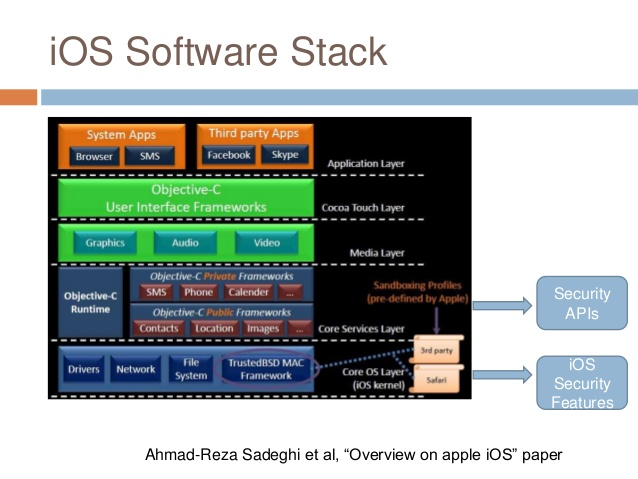
\includegraphics[width=\textwidth]{iOS_stack}
	\centering
	\caption{iOS Software Stack\cite{ios_stack}} 
\end{figure}

\FloatBarrier
\subsubsection{Application structure and components}
iOS applications are distributed via IPA files which are basically archives that have the .ipa extension. Uncompressing the archive reveals the following folder structure \ref{fig_ipa_structure}.
The Payload folder contains the iOS application bundle which is a folder with the applications name and suffixed with the .app extension, in this example its AppName.app.\\
AppName.app contains application binary, static resource files and additional application metadata. The iTunesArtwork file is a Portable Network Graphics (PNG) file that is used as the apps icon in iTunes and the App Store.\\
The iTunesMetadata.plist contians application meta-data such as developers name, bundle identifier and copyright information \cite{Tyrone:2015:MAHH}.
\begin{figure}[h] \label{fig_ipa_structure}
	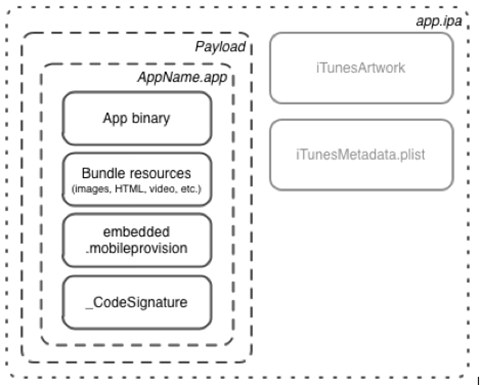
\includegraphics[width=\textwidth]{ipa_structure}
	\centering
	\caption{iOS Software Stack\cite{ipa_structure}} 
\end{figure}
\FloatBarrier
 
\subsubsection{Security model}
iOS has been designed with security at its core. The hardware and software are designed to work in tandem to provide maximum security without compromising on user experience. Apple has published a document detailing the iOS security internals\cite{apple_ios_security_internals} and its salient features are summarised below.
\paragraph{\textbf{Security Architecture}}
Security in iOS is built into the hardware and software stack. Fig \ref{fig_ios_security_arch} shows us various components that make up the security architecture.\\
\begin{itemize}
	\item[]{Secure Boot: Each component of the boot chain is cryptographically signed by Apple to ensure its integrity. If any component of the boot process fails the chain of trust verification, the boot process is aborted and the device enters DFU (Device Firmware Upgrade) mode. The device must then be restored to factory default settings by connecting to iTunes.\\
	At the start of the boot process, the processor executes code from read-only Boot ROM. The Boot ROM is an immutable section of code that contains the Apple Root CA public key. The Boot ROM along with the public key is laid down during the chip fabrication process and is trusted implicitly. The Low-Level Bootloader (LLB) is the next component in the boot chain to be loaded once its signature has been verified by the Boot ROM. Once the LLB has finished executing it verifies and loads the next-stage bootloader, iBoot which in turn verifies and loads the iOS kernel.\\
	The secure boot chain ensures the integrity of low level components to prevent tampering and allows iOS to run only on validated Apple devices.}
	\item[]{System Software Authorization: This is a process used by iOS to upgrade the device with software updates and security patches. This process also prevents devices from being downgraded to older version so as to exploit a vulnerability in an unpatched version.\\
	System Software Authorization is done either via iTunes where a full copy of iOS is downloaded and installed, or over the air (OTA) updates where only affected components are downloaded and installed. During the upgrade the device connects to the Apple installation authorization server and sends it a list of cryptographic measurements for each component being upgraded, a random nounce for prevent replay attacks and the device's unique ID (ECID). The authorization server validates the list of measurements to check if upgrades are permitted. It then adds the ECID to the measurement and signs the result. Signed upgrades are then sent to the device from the server.\\
	The boot time chain-of-trust evaluation verifies that the signature comes from Apple and that the measurements of the items loaded from the disk, combined with the ECID match what was sent by the server.}
	\item[]{Secure Enclave: The Apple A7 and later A-series processors have a coprocessor fabricated in called the Secure Enclave. The coprocessor has its own secure boot process and personalized software upgrade process. It provides all cryptographic operations for Data Protection key management and maintains the integrity of Data Protection even if the kernel is compromised.\\
	It uses encrypted memory and has a built in random number generator. Communication with the application processor is achieved via an isolated interrupt-driven mailbox and shared memeory data buffers. Each Secure Enclave chip is provisioned with its own UID (unique ID) during fabrication and is inaccessible to other parts of the system. On system boot up an ephemeral key is created, entangled with its UID and used to encrypt the Secure Enclave's portion of memory space. Also the data saved to the file system by Secure Enclave is encrypted with a key entangled with the UID and an anti-replay counter.}
	\item[]{Touch ID: This is the fingerprint sensing technology that makes secure access faster and easier. Touch ID although not a replacement for passcodes overcomes the inconvenience of having to frequently enter long passcodes to unlock the device.\\
	Touch ID is a form of user authentication that can also be used to approve purchases from the iTunes Store, the App Store and the iBoot Store.}
\end{itemize}
\begin{figure}[h] \label{fig_ios_security_arch}
	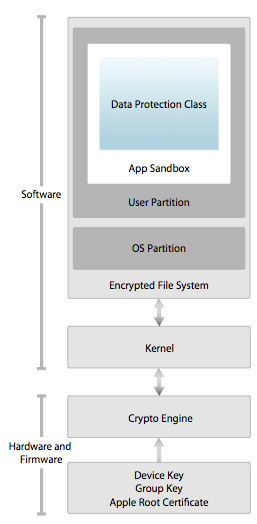
\includegraphics{ios_security_arch}
	\centering
	\caption{iOS security architecture diagram\cite{apple_ios_security_internals}} 
\end{figure}
\FloatBarrier
\paragraph{\textbf{Encryption and Data protection}}
Even if the underlying security infrastructure is compromised, iOS has additional encryption and data protection features to safeguard user data. These features are summarised below
\begin{itemize}
	\item[]{Hardware security features: }
	\item[]{File Data Protection: }
	\item[]{Passcodes:}
	\item[]{Data Protection Classes:}
	\item[]{Keychain data protection: }
	\item[]{Keybags: }
\end{itemize}
\paragraph{\textbf{App security}}
Application security is critical for any smartphone security model and iOS is no exception. iOS ensures that apps are signed and verified and are sandboxed to protect user data. The salient features of app security are summarised below.
\begin{itemize}
	\item[]{App code signing: }
	\item[]{Runtime process security: }
	\item[]{Extensions: }
	\item[]{App Groups: }
	\item[]{Data Protection in apps: }
\end{itemize}

\subsubsection{Current malware landscape}
Although an overwhelming majority of smartphone malware targets Android. There have been a few malware families targeting iOS \cite{current_ios_malware}\cite{ios_malware_exists}. As iOS imporves its market share we predict an increase in malware families targeting iOS.

\begin{itemize}
	\item[]{\textbf{2009:}Trapsms, MobileSpy, Ikee/Eeki, Toires}
	\item[]{\textbf{2010:}LBTM}
	\item[]{\textbf{2011:}iKeyGuard}
	\item[]{\textbf{2012:}FindCall}
	\item[]{\textbf{2013:}Riskware/Killmob}
	\item[]{\textbf{2014:}AdThief/Spad, SSLCreds, Unfold Baby Panda}
	\item[]{\textbf{2015}PawnStorm.A, PawnStrom.B, }
\end{itemize}

\subsection{Others}
Brief discussion on Windows Phone and Blackberry.
\subsubsection{Windows Phone}
\subsubsection{Blackberry OS}


\section{Malware Analysis Process} \label{process}
In this section we look at the goals of malware analysis and what are the question that need to be answered in the analysis report. We also present our generalized approach to analysing malware on smartphones and a potential report template to document the analysis.

\subsection{Goals of Malware Analysis}
The goal of malware analysis is to allow us to answer the following questions \cite{kris:practical_malware_analysis}.
\begin{itemize}
	\item[]{\textbf{What is the purpose of the malware?}}
	\item[]{\textbf{How did it infect the system?}}
	\item[]{\textbf{Who are the attackers and what are the resources at their disposal?}}
	\item[]{\textbf{What did it steal?}}
	\item[]{\textbf{How long has it been here?}}
	\item[]{\textbf{What are the capabilities of this malware?}}
	\item[]{\textbf{How do we identify this malware in the future?}}
\end{itemize}
Malware examination is composed of simple and complex tasks. These tasks can be broadly categorized as into four stages\cite{zeltser:analysis_stages}. These four stages are illustrated in \ref{fig_malware_analysis_stages} as a pyramid. At the bottom of the pyramid we have the easier tasks such which can be done by open source or commercially available tools but offers limited insight into the malware being analysed. As we move higher up the pyramid, the analysis gets more involved requiring a lot more effort and specialized skill set.
\begin{figure}[h] \label{fig_malware_analysis_stages}
	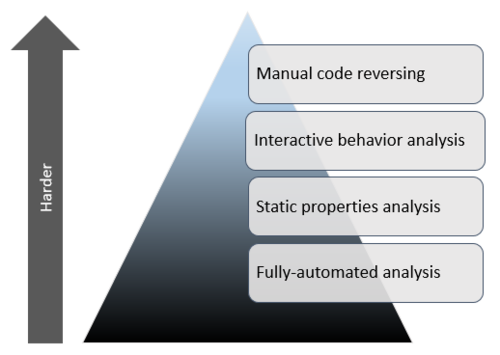
\includegraphics[width=\textwidth]{stages_of_malware_analysis}
	\centering
	\caption{Four stages of malware analysis\cite{zeltser:analysis_stages}} 
\end{figure}
\FloatBarrier 

The four stages can be summarised as follows
\begin{enumerate}
	\item{\textbf{Fully-automated analysis:} This is the easiest stage of malware analysis. It involves scanning the suspected sample with automated tools. These tools are designed to analyse a large number of samples and identify the ones that are potentially malicious. This saves the analyst time in having to manually analyse each sample. However these tools are not absolutely accurate and there can be cases of false-negatives and false-positives.}
	\item{\textbf{Static properties analysis:} This stage invlolves examining the sample without having to actually execute the code. This include analysing strings embedded into the file, header details, hashes, embedded resources, packer signatures, metadata such as the creation date, permissions requested, signing certificates, etc.}
	\item{\textbf{Interactive behaviour analysis:} This stage involves allowing the sample to execute within an isolated environment to observe its behaviour. This stage allows the analyst to study network communications, file operations, processes execution and utilization of system resources.}
	\item{\textbf{Manual code reversing:} This is the final stage in malware analysis and involves reverse engineering the malware sample and analysing the source code. Code analysis is time consuming and burdensome, however it reveals malware capabilities that might not be observable from behaviour analysis.}	
\end{enumerate}

\subsection{Proposed Method} 
\begin{enumerate}
\item{Utilize online analysis services to analyse the sample. Collect analysis reports.}
\item{Create physical and virtual sandboxes for controlled analysis. The analysis sandbox should be equipped with tools to capture network traffic, perform application tracing and data extraction.}
\item{Decompile the application for static analysis. Review the permissions requested, bundled application resources, application strings and malicious patterns in the source code.}
\item{Deploy the sample into the sandbox and observe and record its behaviour.}
\item{Generate a report to summarize the analysis and document artefacts of interest.}
\end{enumerate}

\subsection{Guidelines to creating sandboxes}
System and network isolation
\subsection{Guidelines to static analysis}
What to look for in static analysis
\subsection{Guidelines to dynamic analysis}
What to observe in dynamic analysis
\subsection{Generating an analysis report}
The malware analysis report typically consists of the following sections \cite{zeltser:malwarereport} \cite{soni:malware_report}.
\begin{itemize}
	\item[]{\textbf{Executive Summary:} This section should summarise and highlight the key-points of the analysis. The reader of the report should get a gist of the specimens nature, capabilities, mode of infection and other relevant characteristics.}
	\item[]{\textbf{Identification:} This should include name, size, hashes (MD5, SHA-1 and Fuzzy hashes), packer information,  obfuscator information, known aliases if any, etc.}
	\item[]{\textbf{Capabilities:} This section should describe the capabilities of the malware such as permissions requested and used, data leakage, interaction with the attacker, analysis evasion mechanism, etc.}
	\item[]{\textbf{Dependencies:} This includes any network or file resources that the malware is dependent on for its execution, minimum and maximum version of operating system and other platform dependencies.}
	\item[]{\textbf{Behavioural and Code analysis findings:} This section documents the observations made during behavioural and code analysis. }
	\item[]{\textbf{Supporting data:} This consists of log files, screenshots, network traffic captures, function listings, string excerpts and other artefacts that support the investigation.}
	\item[]{\textbf{Incident Recommendations:} This is section provides indicators for detecting the malware on other systems.}
\end{itemize}

\section{Analysing Android Malware} \label{android_malware_analysis}
This section provides an implementation of the proposed malware analysis for android malware.
\subsection{Sandbox creation}
We describe the creation of physical and virtual sandboxes. This includes configuring network proxies, tools for data extraction and application tracing.
\subsection{Static analysis}
We describe the various tools used for static analysis and what to look for.
\subsection{Dynamic analysis}
We allow our sample to run in the sandbox and record its behaviour.
\subsection{Report generation}
Creating a report for our findings.
\subsection{Case study}
We walk through the analysis of some android malware samples and generate a report.

\section{Limitations}
This section discusses the limitations with the proposed method of malware analysis and possible ways to work around them.
\subsection{analysis evasion techniques}
\subsection{detection of colluding apps}
\subsection{Limitations of analysis tools}

\section{Conclusion}
Review the objectives of the project i.e. discussing the two most popular smartphone platforms and surveying the malware landscape targeting these platforms. Address the secondary objectives of the project.

\bibliographystyle{plain}
\bibliography{bibliography}
\end{document}
